% \section{Suggested Processing Algorithm}
% \label{app:processing_algorithm}
% An idea for minimizing temporarily storage of collected data is to apply the divide-and-conquer technique:
% \begin{itemize}
%     \item Define a static length of a data collection array (or other data structure)
%     \item When the array is full call online processing on that array asynchronously and continue data collecting into the same array
%     \item The result of each processing will be saved as one element in a new intermediate array with same static length as the first array
%     \item This processing strategy continues until the data collection is finished
% \end{itemize}

% Using this algorithm the temporarily storage will have the total space of $O(m*log_m(n))$, and the time consumption of the processing will be $\sum_{i=1}^{log_m(n)}{m^i}$, but parted into $\sum_{i=0}^{log_m(n)-1}{m^i}$ asynchronous calls <<Apply Tactics>>. The larger value the m variable have the more improved the runtimes get.

% \textbf{Example}
% Given $m_1 = 20$ elements and $m_2 = 3$ elements on a total of 8000 elements.
% Space consumption: 
% \begin{itemize}
%     \item $O(m_1*log_{m_1}(n)) = 20*3 = 60$ elements
%     \item $O(m_2*log_{m_2}(n)) = 3*8 = 24$ elements
% \end{itemize}

% Time consumption:
% \begin{itemize}
%     \item $\sum_{i=1}^{log_{m_1}(n)}{m_1^i} = 20+400+8000 = 8420$ elements to process
%     \item $\sum_{i=0}^{log_{m_1}(n)-1}{m_1^i} = 1+20+400 = 421$ process calls
%     \item $\sum_{i=1}^{log_{m_2}(n)}{m_2^i} = 3+9+27+81+243+729+2187+6561 = 9840$ elements to process
%     \item $\sum_{i=0}^{log_{m_2}(n)-1}{m_2^i} = 1+3+9+27+81+243+729+2187 = 3280$ process calls
% \end{itemize}

% This shows the size of m have the largest effect on number of process calls.
% Without this algorithm the space consumption would be $O(n) = 8000$ elements and time consumption would be $O(n) = 8000$ elements to process within $O(1) = 1$ process call.


%----------------------------------- Interface Figure
\subsection{Interfaces}
\label{app:interfaces}

\begin{figure}[H]
    \centering
    \hspace*{-1.73in}
    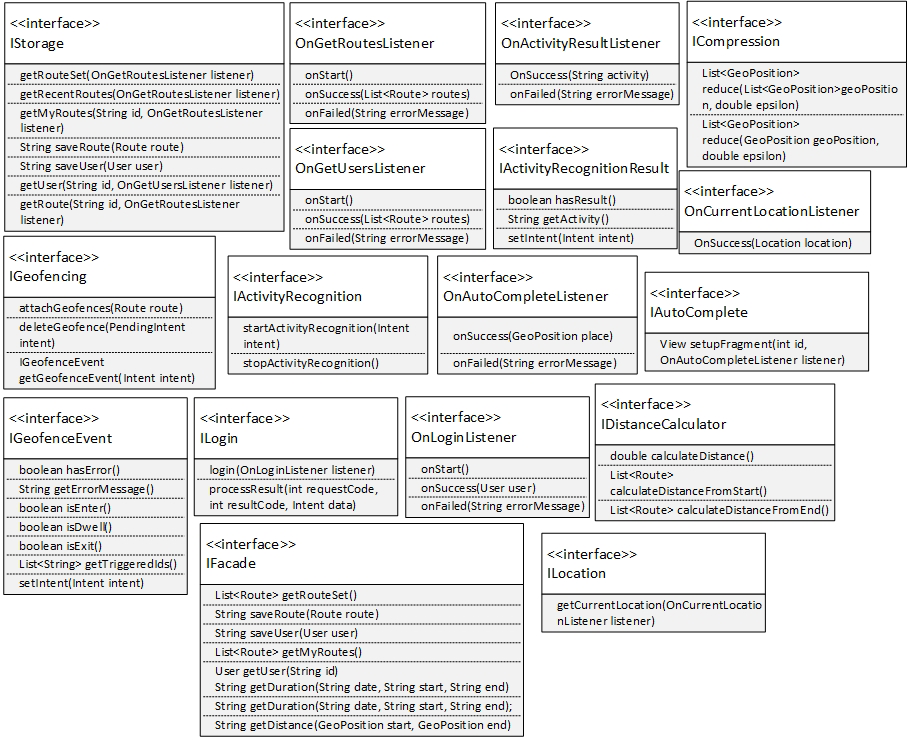
\includegraphics[scale=0.65]{Graphics/Images/Interfaces.png}
    \caption{Class diagram of interfaces}
    \label{fig:interfaces}
\end{figure}


%----------------------------------- Firebase Figures
\subsection{Firebase Structure}

\label{app:firebase_figures}
\begin{figure}[H]
    \centering
    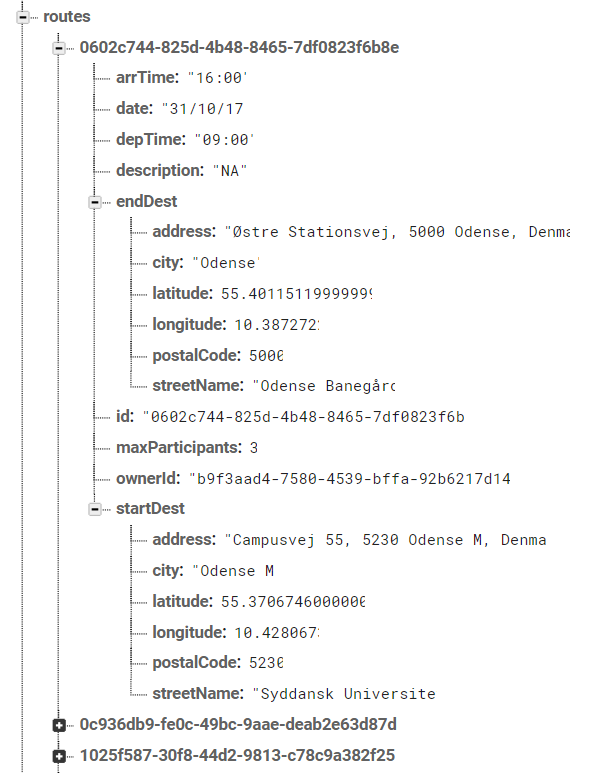
\includegraphics[scale=1.5]{Graphics/Images/firebase_routes.PNG}
    \caption{Route objects in Firebase}
    \label{fig:firebase_routes_appendix}
\end{figure}

\begin{figure}[H]
    \centering
    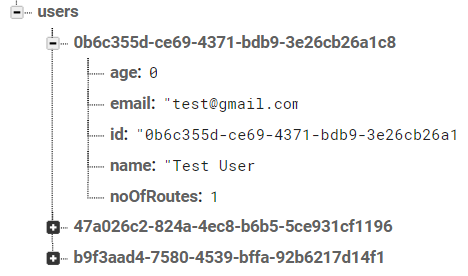
\includegraphics[scale=1.5]{Graphics/Images/firebase_users.PNG}
    \caption{User objects in Firebase}
    \label{fig:firebase_users_appendix}
\end{figure}


%----------------------------------- Compression Figures
\subsection{Compression}
\label{app:compression}

\begin{figure}[H]
    \centering
    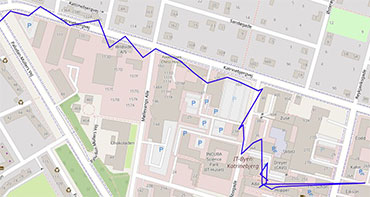
\includegraphics[scale=1.0]{RouteWithOutFilter2.jpg}
    \caption{Without median filter (blue line)}
    \label{fig:route_without_filter_appendix}
\end{figure}

\begin{figure}[H]
    \centering
    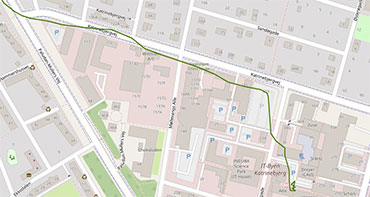
\includegraphics[scale=1.0]{RouteWithFilter2.jpg}
    \caption{With median filter (green line)}
    \label{fig:route_with_filter_appendix}
\end{figure}

\begin{figure}[H]
    \centering
    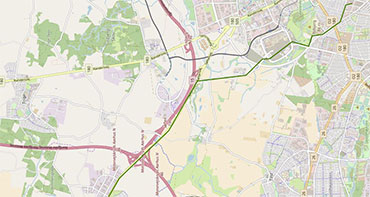
\includegraphics[scale=1.0]{RouteDP2.jpg}
    \caption{Douglas Peucker compression (green line)}
    \label{fig:douglas_peucker_compression_appendix}
\end{figure}

\begin{figure}[H]
\centering
    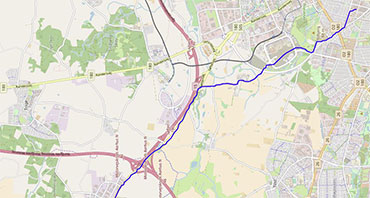
\includegraphics[scale=1.0]{RouteSW2.jpg}
    \caption{Sliding window compression (blue line)}
    \label{fig:sliding_window_appendix}
\end{figure}
